\section{Design}
I decided to write this project in Python with the external library OpenCV, in figure \ref{fig:packages_diagram} can be seen the diagram of the packages with relative classes.
Since I do not use the bounding boxes that are downloaded with the dataset the first thing I need to do is getting a correspondence landmark (using dlib) to valence for each frame of each video, the execution took almost 21 hours so I made possible to save the results as text files.
Each valence ranges from -1 to 1, I explicitly ignored valences $v$ such that $-0.5 \leq v \leq 0.5 $ to minimize noise and rule out uncertain valences, in the end were extracted 136909 landmark-valence tuple.
Is possible for a single frame to contain more than a face as seen in figure \ref{fig:double_face} \footnote{I find bounding boxes less invasive, in this case landmark detects two faces as well.}.
Since the affwild datasets collects videos with foreground faces is reasonable to assume that the face we're interested in is the widest one, hence I pick the one with the largest euclidean distance between the first and last point of the feature points (respectively the lateral commissure of the viewer's left eye and the lower lip).

\begin{figure}
    \centering
    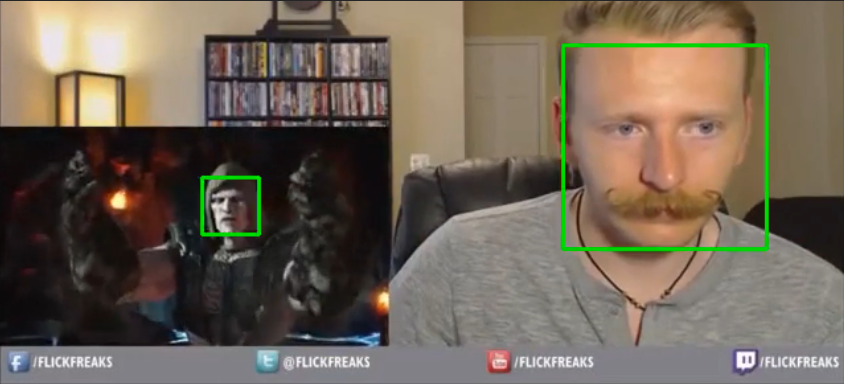
\includegraphics[scale=0.4]{images/309mp4_double_face.png}
    \caption{Two faces detected in the video 309.}
    \label{fig:double_face}
\end{figure}

Valences are saved and read as an array of floats \footnote{datasets/misc/valences.txt} while landmarks are a two dimensional array \footnote{datasets/misc/landmarks.txt}. 
For each face dlib stores landmark points as an array of $[x,y]$ coordinates, to make things more readable - and possibily to make the code faster in corner cases due to caching - I decided to flatten it as a one dimensional vector. 
I don't think this different encoding should change SVM's predictions.

Regarding SVM classification I first used the implementation in OpenCV with bad performances while the Sklearn one is way better. For this reason the demo uses the latter. 
During tests the dataset has been splitted as 80-20 per cent for train and test respectively.  

In the demo instead of directly detecting landmark points I first detect bboxes. 
This may be odd but I noticed how bounding boxes are less accurate than landmark points, detecting less landmarks makes the demo less precise but is smoother for a presentation. 

Both bounding boxes and landmark points were detected through pretained models ~\cite{dataset:haar} ~\cite{dataset:landmark}.

The general structure of classes and packages that were defined can be seen in figure \ref{fig:packages_diagram}, it is all original code except the function \textcode{src.test.Test.plot\_roc} used to plot ROC curves. It has been taken from \href{https://www.codespeedy.com/how-to-plot-roc-curve-using-sklearn-library-in-python/}{here} as commented in the source code.

\begin{figure}
    \centering
    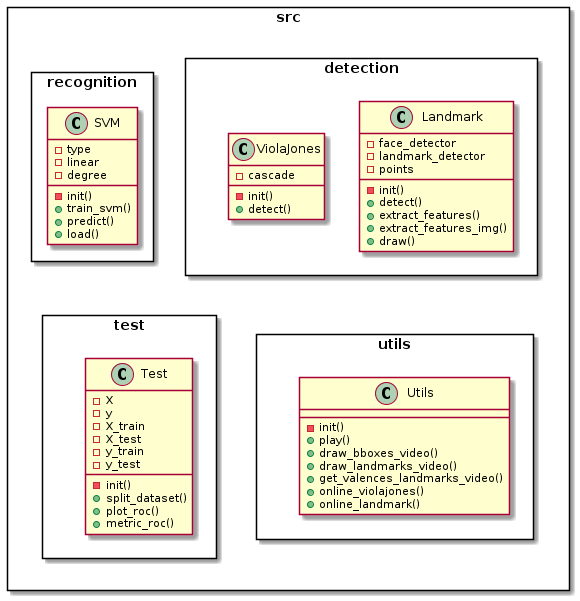
\includegraphics[scale=0.55]{../../diagrams/out/src/classes.png}
    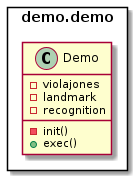
\includegraphics[scale=0.55]{../../diagrams/out/demo/classes.png}
    \caption{Diagram of the packages.}
    \label{fig:packages_diagram}
\end{figure}

Other code that is not original are clearly external functions.
I used the following external librariees:
\begin{itemize}
    \item \textbf{os} To explore the filesystem.
    \item \textbf{re} For regular expressions.
    \item \textbf{fire} To implement command line arguments.
    \item \textbf{numpy} The use of arrays is essential thanks to this faster C implementation.
    \item \textbf{cv2} OpenCV as stated above, it has been used for detection with Haar features and an SVM implementation.
    \item \textbf{dlib} For landmark points since for OpenCV there is still no Python implementation.
    \item \textbf{sklearn} In this library is implemented a more performing SVM classifier than OpenCV's one.
    \item \textbf{joblib} used to save sklearn's SVM model.
\end{itemize}
